\chapter{Вторая глава}
Здесь текст второй главы. Пример с рисунком.

С поставленной задачей генетический алгоритм справился за 50 поколений. Результаты представлены на рисунке~\ref{fig:genetic_envelope}.

\begin{figure}[!ht]
    \centering
    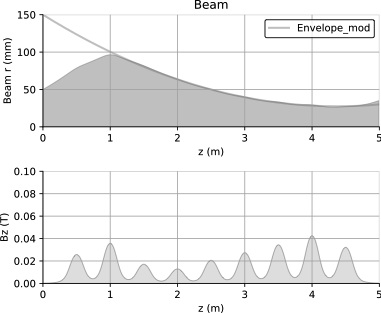
\includegraphics[width=0.65\textwidth]{figures/genetic_envelope_bw.png}
    \caption{Результат восстановления огибающей под заданную 
    и полученное магнитное поле~$B_z(z)$ для 50-го поколения}
    \label{fig:genetic_envelope}
\end{figure}